\section{问题二模型的建立与求解}

\subsection{模型建立}

问题二中园区制氨产能增至72吨/日，制氢氨设备功率按比例线性提升至41.5 MW（ALKEL 20 MW + PEMEL 20 MW + 合成氨装置1.5 MW，产率3.0 t/h）。电氢氨装置只有全额开机和停机两种运行方式，制氨产量从72吨/日起按9吨/日递减至36吨/日。这是一个典型的0-1整数规划问题。

定义0-1变量$x(t) \in \{0,1\}$表示时段$t$是否开机生产：
\begin{equation}
x(t) = \begin{cases}
1, & \text{时段}t\text{开机生产} \\
0, & \text{时段}t\text{停机}
\end{cases} \quad t = 0,1,\ldots,23
\end{equation}

目标为最小化日净电费（购电成本减去售电收益）与运维成本之和：
\begin{equation}
\min \; F = \sum_{t=0}^{23} \bigl[ P_{\mathrm{b}}(t)C_{\mathrm{b}}(t) - P_{\mathrm{s}}(t)C_{\mathrm{s}} + C_{\mathrm{OM}}(t) \bigr] \label{eq:q2_obj}
\end{equation}
当$x(t)=1$时，$P_{\mathrm{prod}}(t)=P_{\mathrm{max}}=41.5$ MW；当$x(t)=0$时，$P_{\mathrm{prod}}(t)=0$。运维成本$C_{\mathrm{OM}}(t) = x(t) \times 5003$元。

约束条件包括功率平衡约束、日产量约束和购售电互斥约束：
\begin{align}
&P_{\mathrm{w}}(t) + P_{\mathrm{pv}}(t) + P_{\mathrm{b}}(t) = P_{\mathrm{L}}(t) + x(t)P_{\mathrm{max}} + P_{\mathrm{s}}(t) \quad \forall t \label{eq:q2_bal} \\
&\sum_{t=0}^{23} x(t) = k,\quad k = Q_{\mathrm{NH_3}}/3 \in \{24,21,18,15,12\} \label{eq:q2_hours} \\
&P_{\mathrm{b}}(t) \ge 0,\; P_{\mathrm{s}}(t) \ge 0,\; P_{\mathrm{b}}(t) \cdot P_{\mathrm{s}}(t) = 0 \quad \forall t
\end{align}

整理为标准整数规划形式：
\begin{align}
\min \; & \sum_{t=0}^{23} \bigl[ C_{\mathrm{b}}(t)\max\{P_{\mathrm{L}}(t) + x(t)P_{\mathrm{max}} - P_{\mathrm{w}}(t) - P_{\mathrm{pv}}(t),\; 0\} \notag \\
&\qquad - C_{\mathrm{s}}\max\{P_{\mathrm{w}}(t) + P_{\mathrm{pv}}(t) - P_{\mathrm{L}}(t) - x(t)P_{\mathrm{max}},\; 0\} + 5003x(t) \bigr] \label{eq:q2_model} \\
\text{s.t.} \quad & \sum_{t=0}^{23} x(t) = k,\; x(t) \in \{0,1\},\; \forall t \notag
\end{align}

\subsection{模型求解}

\textbf{步骤一：确定开机时长。}根据目标日产量$Q_{\mathrm{NH_3}}$，计算所需开机小时数$k = Q_{\mathrm{NH_3}}/3$。72、63、54、45、36吨/日分别对应$k=24,21,18,15,12$小时。

\textbf{步骤二：计算各时段边际成本。}对于每个时段$t=0,\ldots,23$，按以下公式计算相对于不开机而言，开机的边际成本$\Delta C(t)$：
\begin{equation}
\Delta C(t) = \bigl[ C_{\mathrm{on}}(t) - C_{\mathrm{off}}(t) \bigr] + 5003 \label{eq:q2_marginal}
\end{equation}
其中：
\begin{align*}
C_{\mathrm{off}}(t) &=
\begin{cases}
- [P_{\mathrm{w}}(t)+P_{\mathrm{pv}}(t)-P_{\mathrm{L}}(t)] \cdot C_{\mathrm{s}}, & \text{若可再生过剩}\\
[P_{\mathrm{L}}(t)-P_{\mathrm{w}}(t)-P_{\mathrm{pv}}(t)] \cdot C_{\mathrm{b}}(t), & \text{若可再生不足}
\end{cases} \\
C_{\mathrm{on}}(t) &=
\begin{cases}
- [P_{\mathrm{w}}(t)+P_{\mathrm{pv}}(t)-P_{\mathrm{L}}(t)-41.5] \cdot C_{\mathrm{s}}, & \text{若开机后仍过剩}\\
[P_{\mathrm{L}}(t)+41.5-P_{\mathrm{w}}(t)-P_{\mathrm{pv}}(t)] \cdot C_{\mathrm{b}}(t), & \text{若开机后需购电}
\end{cases}
\end{align*}
常数5003元是开机一小时产生的运维费用（ALKEL 20MW$\times$100 + PEMEL 20MW$\times$150 + NH$_3$ 1.5MW$\times$2）。

以$t=12$（12:00-13:00，峰电价0.8024元/kWh）为例：
\begin{align*}
C_{\mathrm{off}}(12) &= -(14.52+46.08-3.26)\times 377.9 = -21\,668\ \text{元} \quad (\text{售电收益})\\
C_{\mathrm{on}}(12) &= -(14.52+46.08-3.26-41.5)\times 377.9 = -5\,985\ \text{元}\\
\Delta C(12) &= (-5\,985) - (-21\,668) + 5\,003 = -10\,680\ \text{元}
\end{align*}
边际成本为负，说明$t=12$开机比停机更省钱（将低价值余电转为氨生产，扣除运维后仍有净收益）。

以$t=19$（19:00-20:00，峰电价0.8024元/kWh）为例：
\begin{align*}
C_{\mathrm{off}}(19) &= (2.12-3.69)\times 0 = 0\ \text{元} \quad (\text{无可再生能源，但净负荷为负})\\
C_{\mathrm{on}}(19) &= (2.12+41.5-3.69)\times 802.4 = 32\,088\ \text{元}\\
\Delta C(19) &= 32\,088 - 0 + 5\,003 = 37\,091\ \text{元}
\end{align*}
边际成本很高，说明$t=19$开机需大量购电，成本极高。

\textbf{步骤三：选择最优时段。}将24个$\Delta C(t)$从小到大排序，选择前$k$个最小的时段开机。以36吨/日（$k=12$）为例，边际成本最低的12个时段集中在10:00-21:00（太阳能充足或风能较好的时段），而夜间和清晨因光伏为零且风电不够支撑满负荷，边际成本较高，因此不开机。

\textbf{步骤四：计算指标和成本。}根据选定的开机方案，计算购售电功率，然后按模型建立部分的公式计算绿电指标和吨氨成本。各产量结果如\cref{tab:q2_typical}所示。

\begin{table}[H]
\centering
\caption{典型场景各产量运行指标}
\label{tab:q2_typical}
\begin{tabular*}{\textwidth}{@{\extracolsep{\fill}}ccccccc}
\toprule[1.5pt]
产量(t/d) & 时长(h) & 成本(元/吨) & 自用比例 & 绿电比例 & 上网比例 & 达标 \\
\midrule[1pt]
72 & 24 & 6219 & 86.5\% & 53.3\% & 6.7\% & $\checkmark$ \\
63 & 21 & 5328 & 84.3\% & 59.7\% & 7.8\% & $\checkmark$ \\
54 & 18 & 4591 & 80.2\% & 67.3\% & 9.9\% & $\checkmark$ \\
45 & 15 & 3945 & 51.0\% & 66.7\% & 24.5\% & $\times$ \\
36 & 12 & 3192 & 10.5\% & 59.7\% & 44.7\% & $\times$ \\
\bottomrule[1.5pt]
\end{tabular*}
\end{table}

\cref{tab:q2_typical}展示了各产量下的成本与绿电指标。随着产量降低，运行小时数减少，购电量也随之下降，使得吨氨成本从72 t/d的6219元/吨降至36 t/d的3192元/吨。然而，低产量下自发自用比例也大幅下滑——36 t/d时仅10.5\%（不满足60\%要求），而上网比例达到44.7\%（不满足20\%要求），说明离散调节下低产工况难以兼顾经济性与绿电指标。

为进一步分析开机策略，根据各产量的最优开机时段绘制甘特图如\cref{fig:q2_gantt}所示。

\begin{figure}[H]
\centering
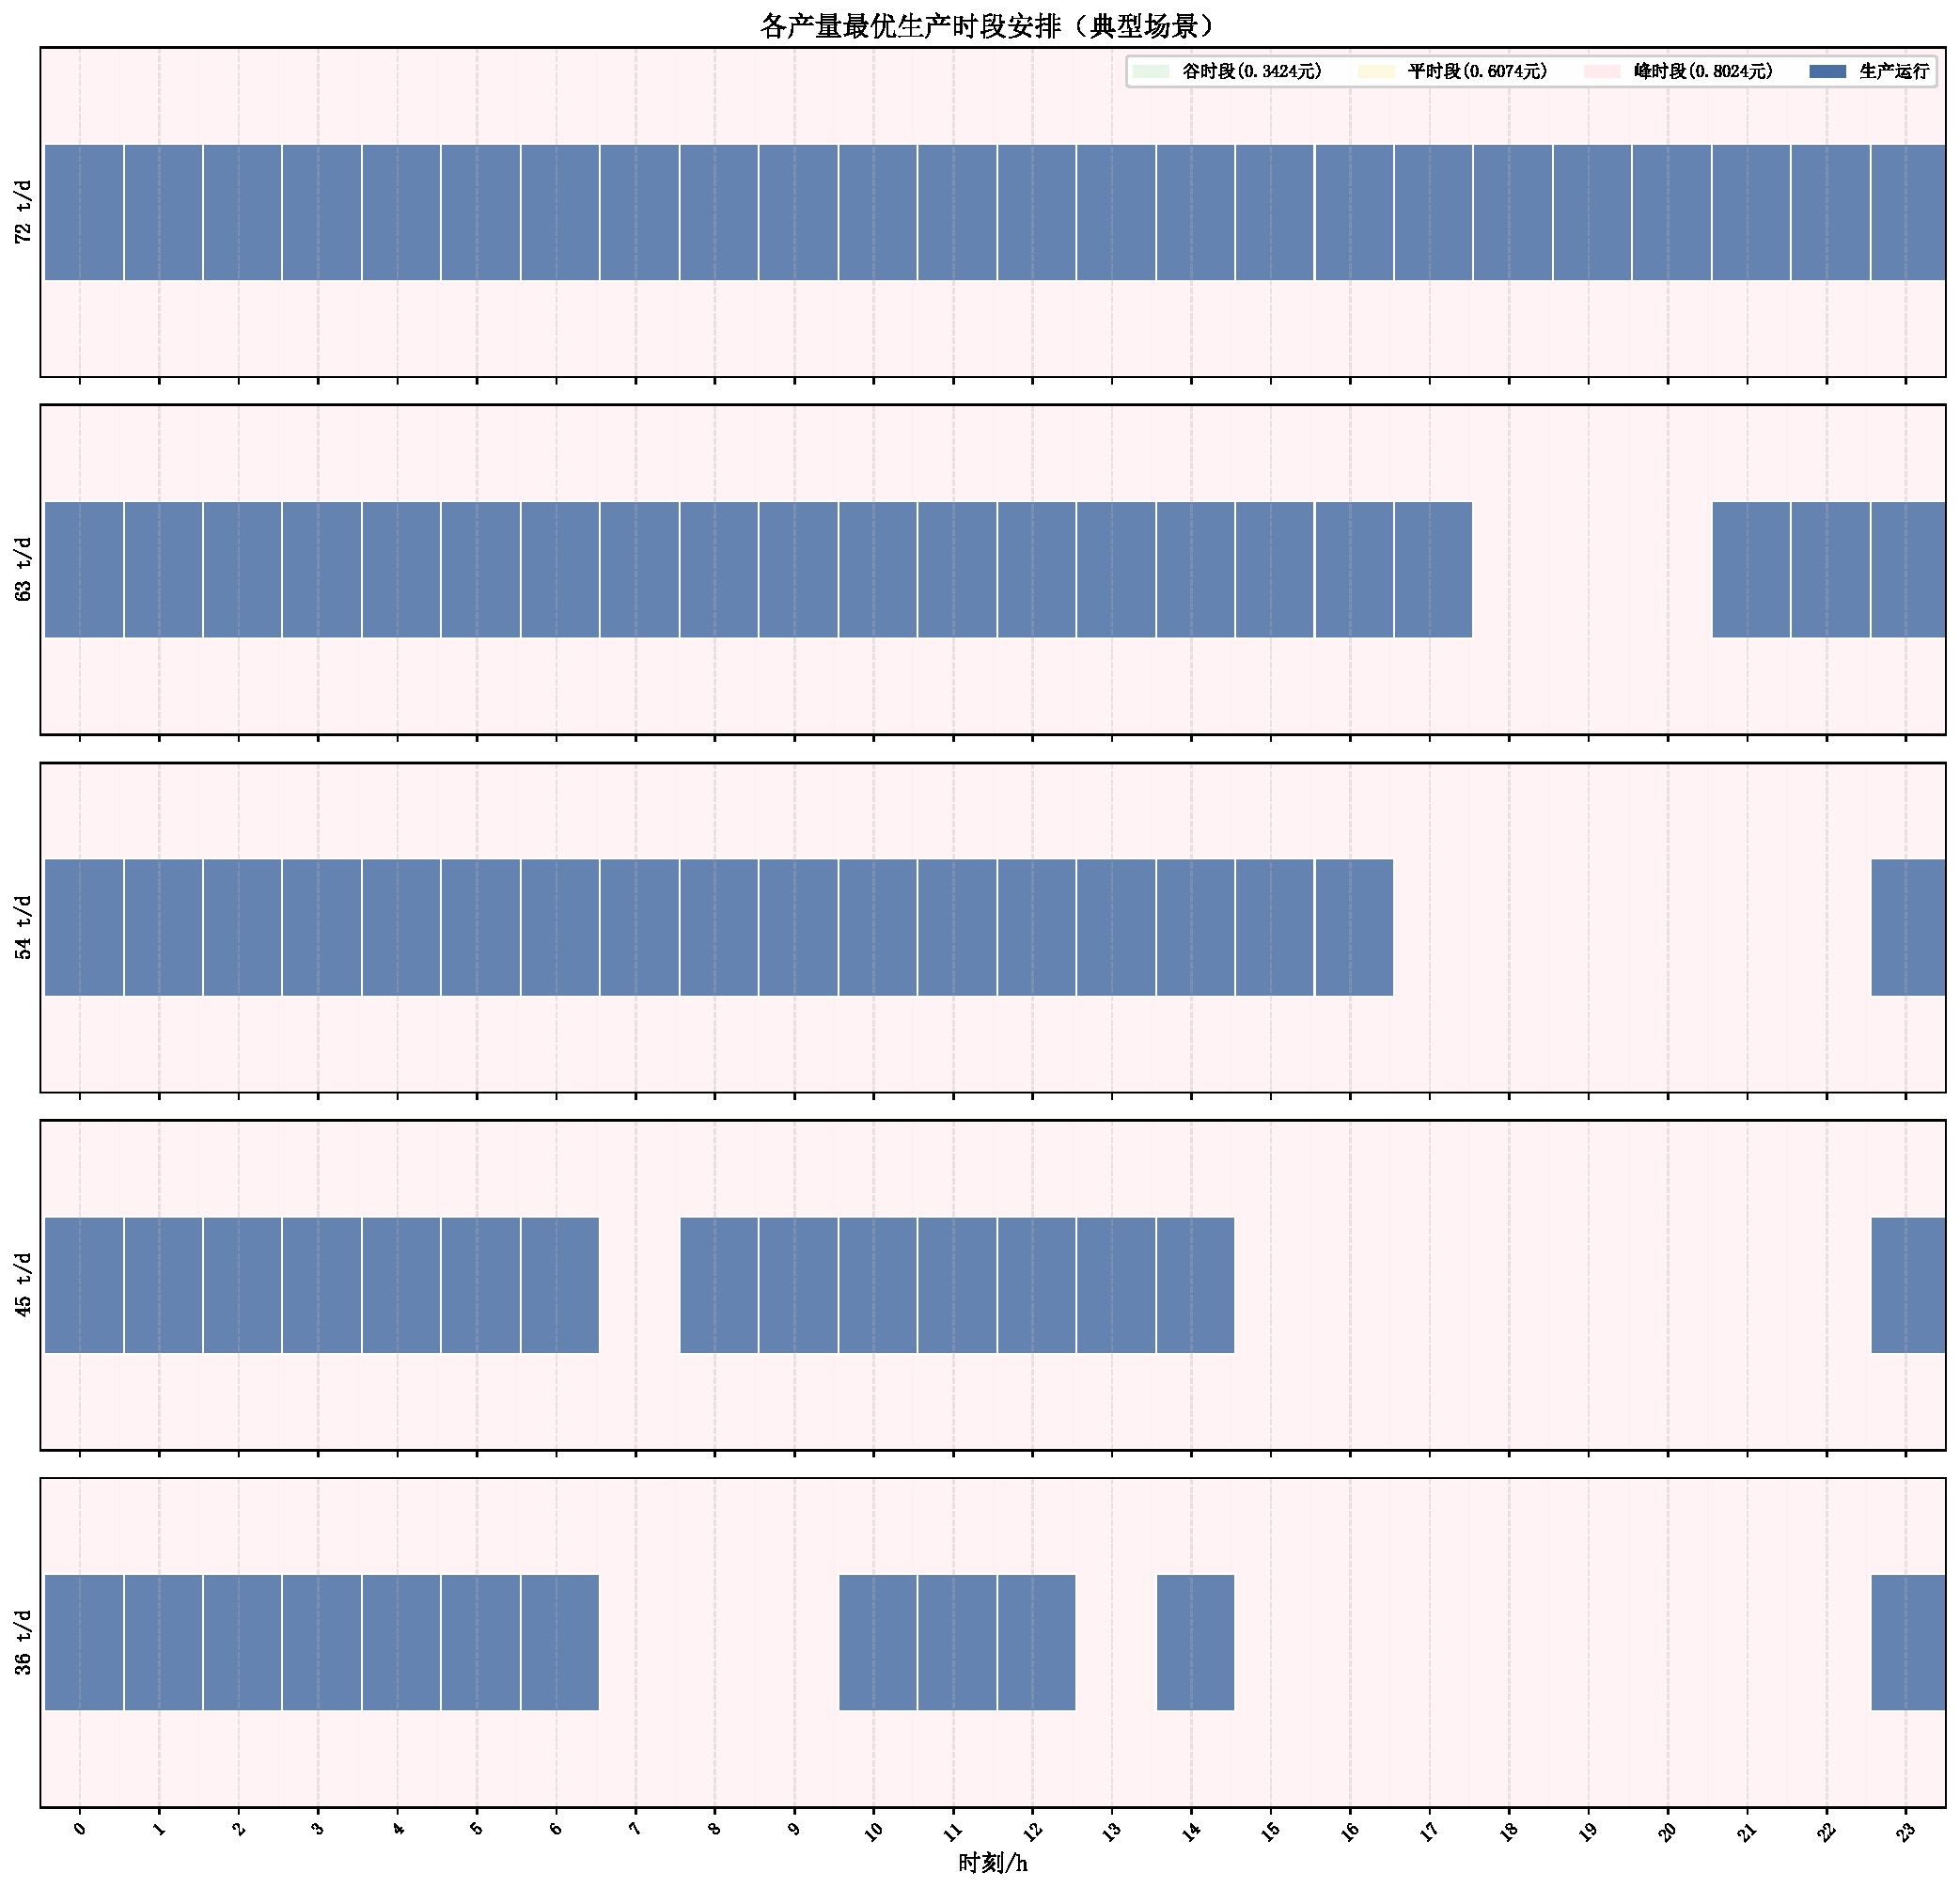
\includegraphics[width=\textwidth]{../figures/q2/fig4_gantt.pdf}
\caption{各产量最优生产时段安排}
\label{fig:q2_gantt}
\end{figure}

\cref{fig:q2_gantt}展示了各产量下最优的24小时开机方案（蓝色条）与电价时段（谷时段绿色、平时段黄色、峰时段粉红）的关系。72 t/d需满发24h，无法选择；63 t/d优先关停了18:00-20:00峰时段（此时光伏归零而负荷攀升，购电成本高达0.8024元/kWh）；54 t/d、45 t/d、36 t/d依次继续关停成本最高的时段，优先保留谷电价时段（0.3424元/kWh）和光伏大发的中午时段。这表明边际成本排序算法倾向于在低价时段和高可再生时段安排生产，有效降低了购电成本。

由各产量的成本和绿电指标数据得到\cref{fig:q2_cvp}。

\begin{figure}[H]
\centering
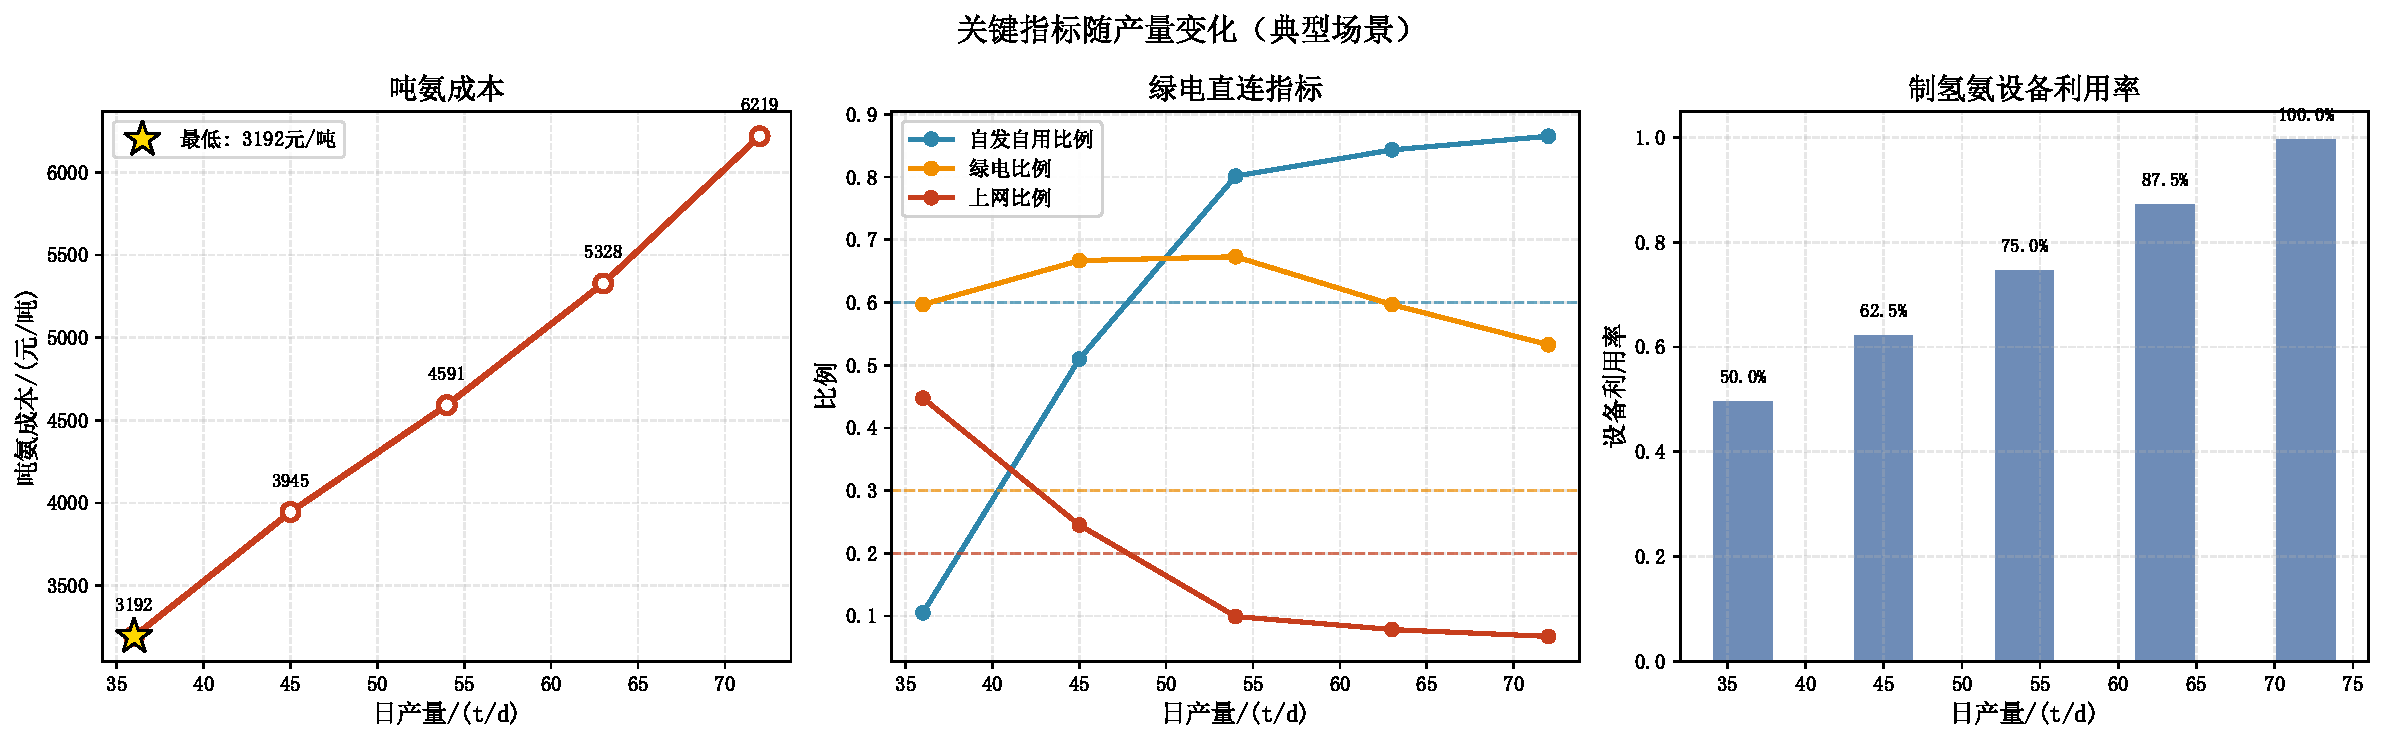
\includegraphics[width=\textwidth]{../figures/q2/fig5_cost_vs_production.pdf}
\caption{关键指标随产量变化}
\label{fig:q2_cvp}
\end{figure}

\cref{fig:q2_cvp}包含三个子图。(a)吨氨成本曲线：从72 t/d的6,219元/吨单调下降至36 t/d的3,192元/吨，降幅约49\%。这是因为低产量下设备运行时间短，购电费用减少、售电收益增加，单位成本被摊薄。(b)绿电指标曲线：自用比例在72-54 t/d时稳定在80\%以上，但45 t/d时骤降至51.0\%（低于60\%要求），36 t/d时进一步降至10.5\%。上网比例在54 t/d时仅9.9\%（达标），45 t/d时升至24.5\%（超标）。这表明离散调节下低产量时大部分可再生电力被上网出售而非自用，导致指标恶化。(c)设备利用率：随产量线性降低，从100\%降至50\%。

以上分析均基于典型日风光出力场景。然而园区实际运行中风光出力具有显著的随机波动性——风电可能全天低于额定功率的10\%，光伏可能因多云天气出力减半。为全面评估离散调节方案在不同天气条件下的表现，将附件3的6种风电场景与附件4的4种光伏场景进行两两组合，共得到24种风光出力场景（如S1风1光1、S2风1光2、…、S24风6光4）。对每种场景重复上述边际成本优化，计算各产量水平下的吨氨成本，绘制热力图如\cref{fig:q2_heatmap}所示。

\begin{figure}[H]
\centering
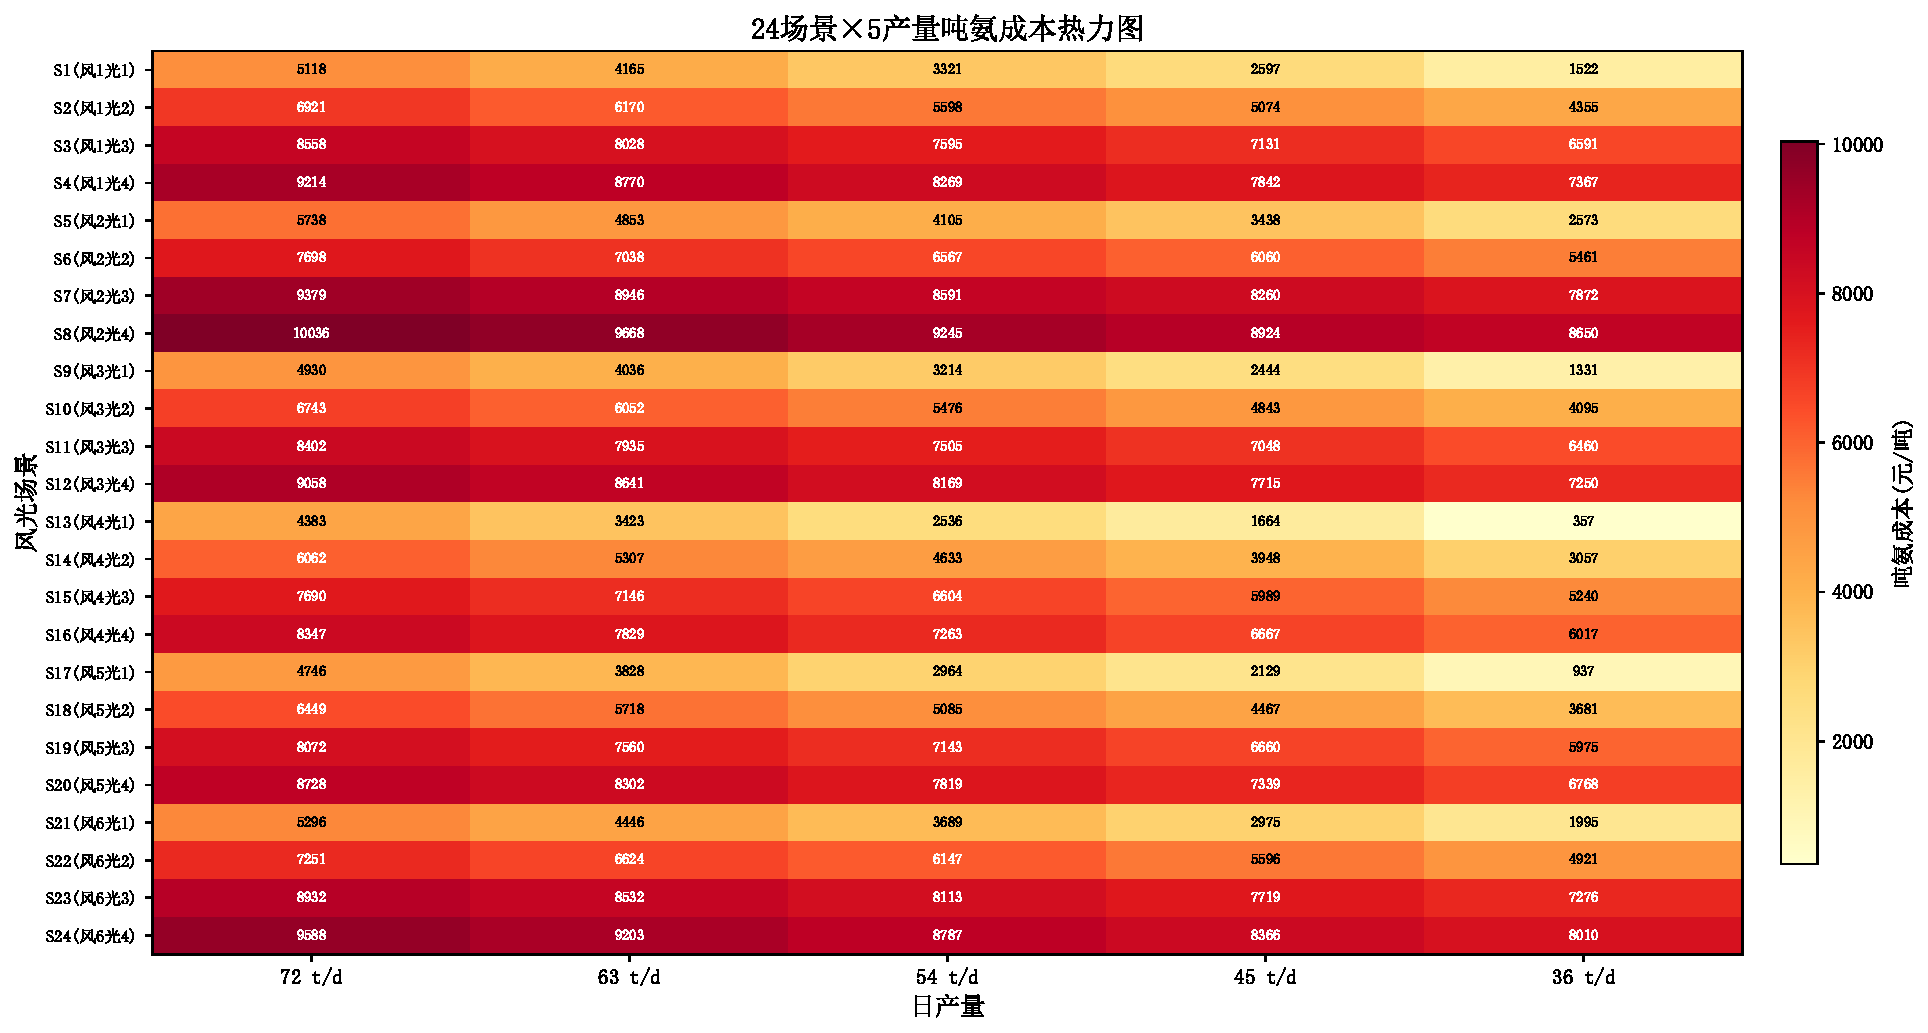
\includegraphics[width=\textwidth]{../figures/q2/fig6_heatmap.pdf}
\caption{24场景$\times$5产量吨氨成本热力图}
\label{fig:q2_heatmap}
\end{figure}

\cref{fig:q2_heatmap}中每一行代表一种风光场景，每一列代表一个产量水平，颜色深浅反映吨氨成本高低。场景S8（风2光4，风电和光伏均偏低）在所有产量下成本均为最高，原因是该场景可再生发电总量少，需大量网购高价电力；场景S13（风4光1，风电高光伏中等）成本最低，因为风电在夜间和全天持续出力。高产量时各场景间成本差异较小（约1,000-2,000元/吨），低产量时差异显著增大（可达5,000元/吨以上），说明低产量下风光条件对经济性的影响更为敏感。

各产量下24种场景的绿电指标达标情况统计如\cref{fig:q2_compliance}所示。

\begin{figure}[H]
\centering
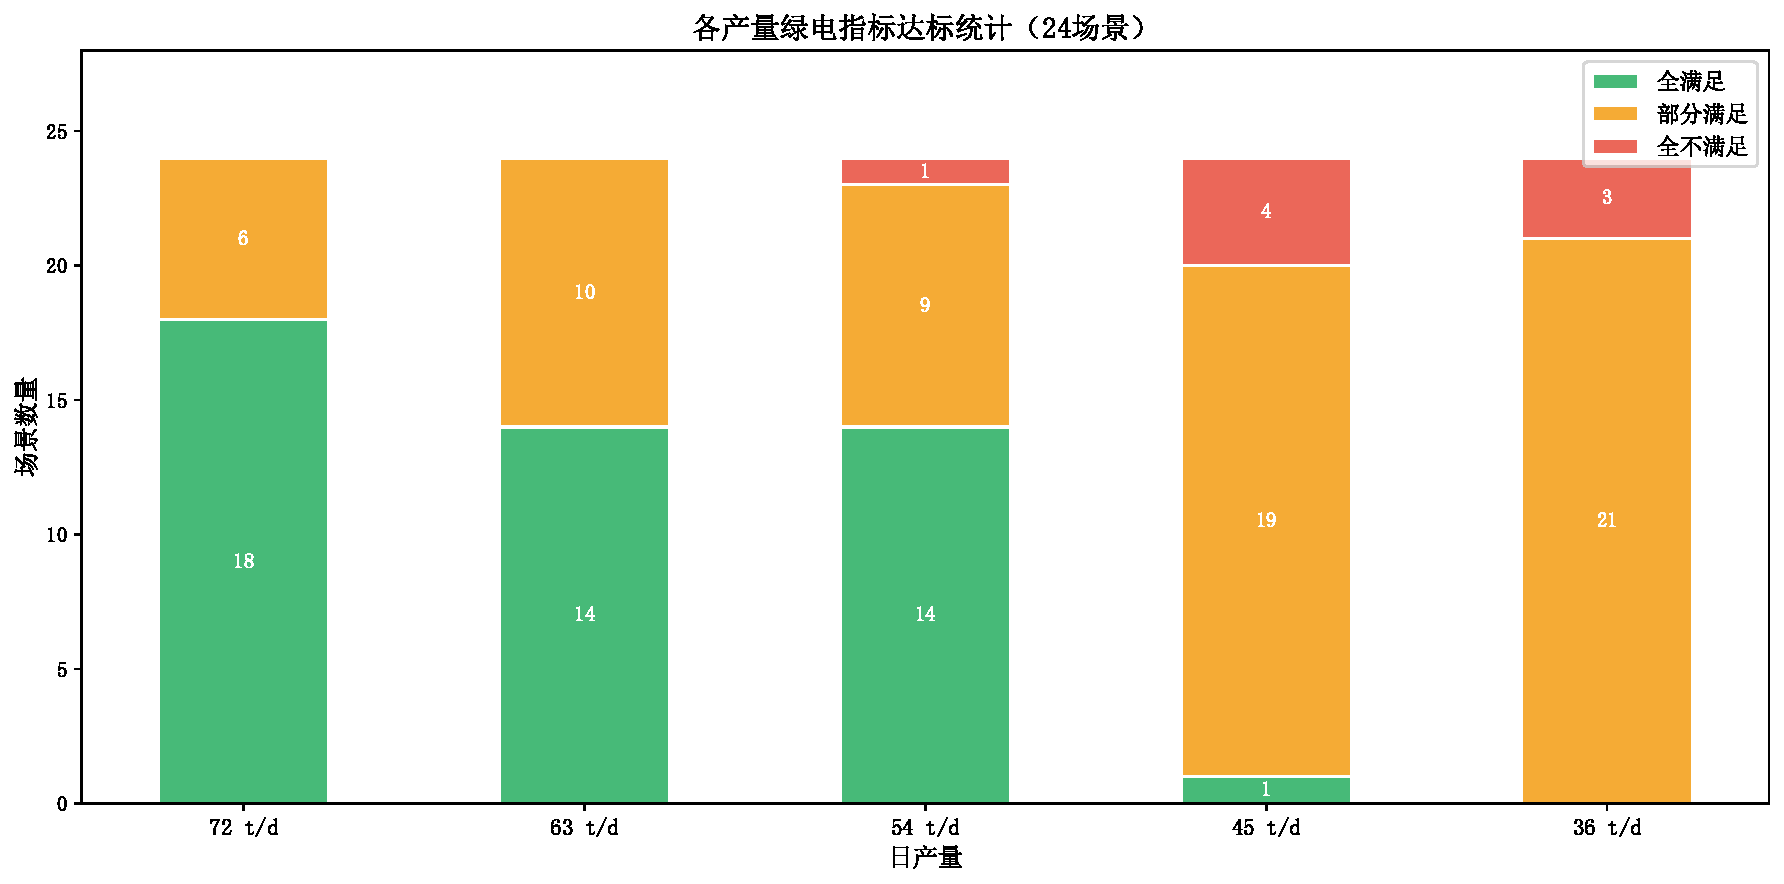
\includegraphics[width=\textwidth]{../figures/q2/fig7_compliance.pdf}
\caption{各产量绿电指标达标统计}
\label{fig:q2_compliance}
\end{figure}

\cref{fig:q2_compliance}按全满足（绿）、部分满足（黄）、全不满足（红）三类统计了24场景的达标情况。72 t/d时18个场景全满足、6个部分满足，表现最好；63 t/d和54 t/d分别有14个全满足，仍属良好；45 t/d时仅1个全满足、19个部分满足、4个全不满足，急剧恶化；36 t/d时0个全满足、21个部分满足、3个全不满足。这说明离散调节下产量降至45 t/d及以下时，即使针对不同风光场景优化调度，也无法使大多数场景的绿电指标达标。根本原因是开机时长过短导致可再生自用电量太少、上网比例过高。
